
\documentclass[border=8pt, multi, tikz]{standalone} 
\usepackage{import}
\subimport{../../layers/}{init}
\usetikzlibrary{positioning, calc, 3d} % Added 'calc' for coordinate calculations

\usetikzlibrary{3d} %for including external image 

\def\ConvColor{rgb:yellow,5;red,2.5;white,5}
\def\ConvReluColor{rgb:yellow,5;red,5;white,5}
\def\PoolColor{rgb:red,1;black,0.3}
\def\UnpoolColor{rgb:blue,2;green,1;black,0.3}
\def\FcColor{rgb:blue,5;red,2.5;white,5}
\def\FcReluColor{rgb:blue,5;red,5;white,4}
\def\SoftmaxColor{rgb:magenta,5;black,7}   
\def\SumColor{rgb:blue,5;green,15}

\newcommand{\copymidarrow}{\tikz \draw[-Stealth,line width=0.8mm,draw={rgb:blue,4;red,1;green,1;black,3}] (-0.3,0) -- ++(0.3,0);}

\begin{document}
\begin{tikzpicture}
\tikzstyle{connection}=[ultra thick,every node/.style={sloped,allow upside down},draw=\edgecolor,opacity=0.7]
\tikzstyle{copyconnection}=[ultra thick,every node/.style={sloped,allow upside down},draw={rgb:blue,4;red,1;green,1;black,3},opacity=0.7]


\node[canvas is zy plane at x=0] (input) at (-3,0,0) {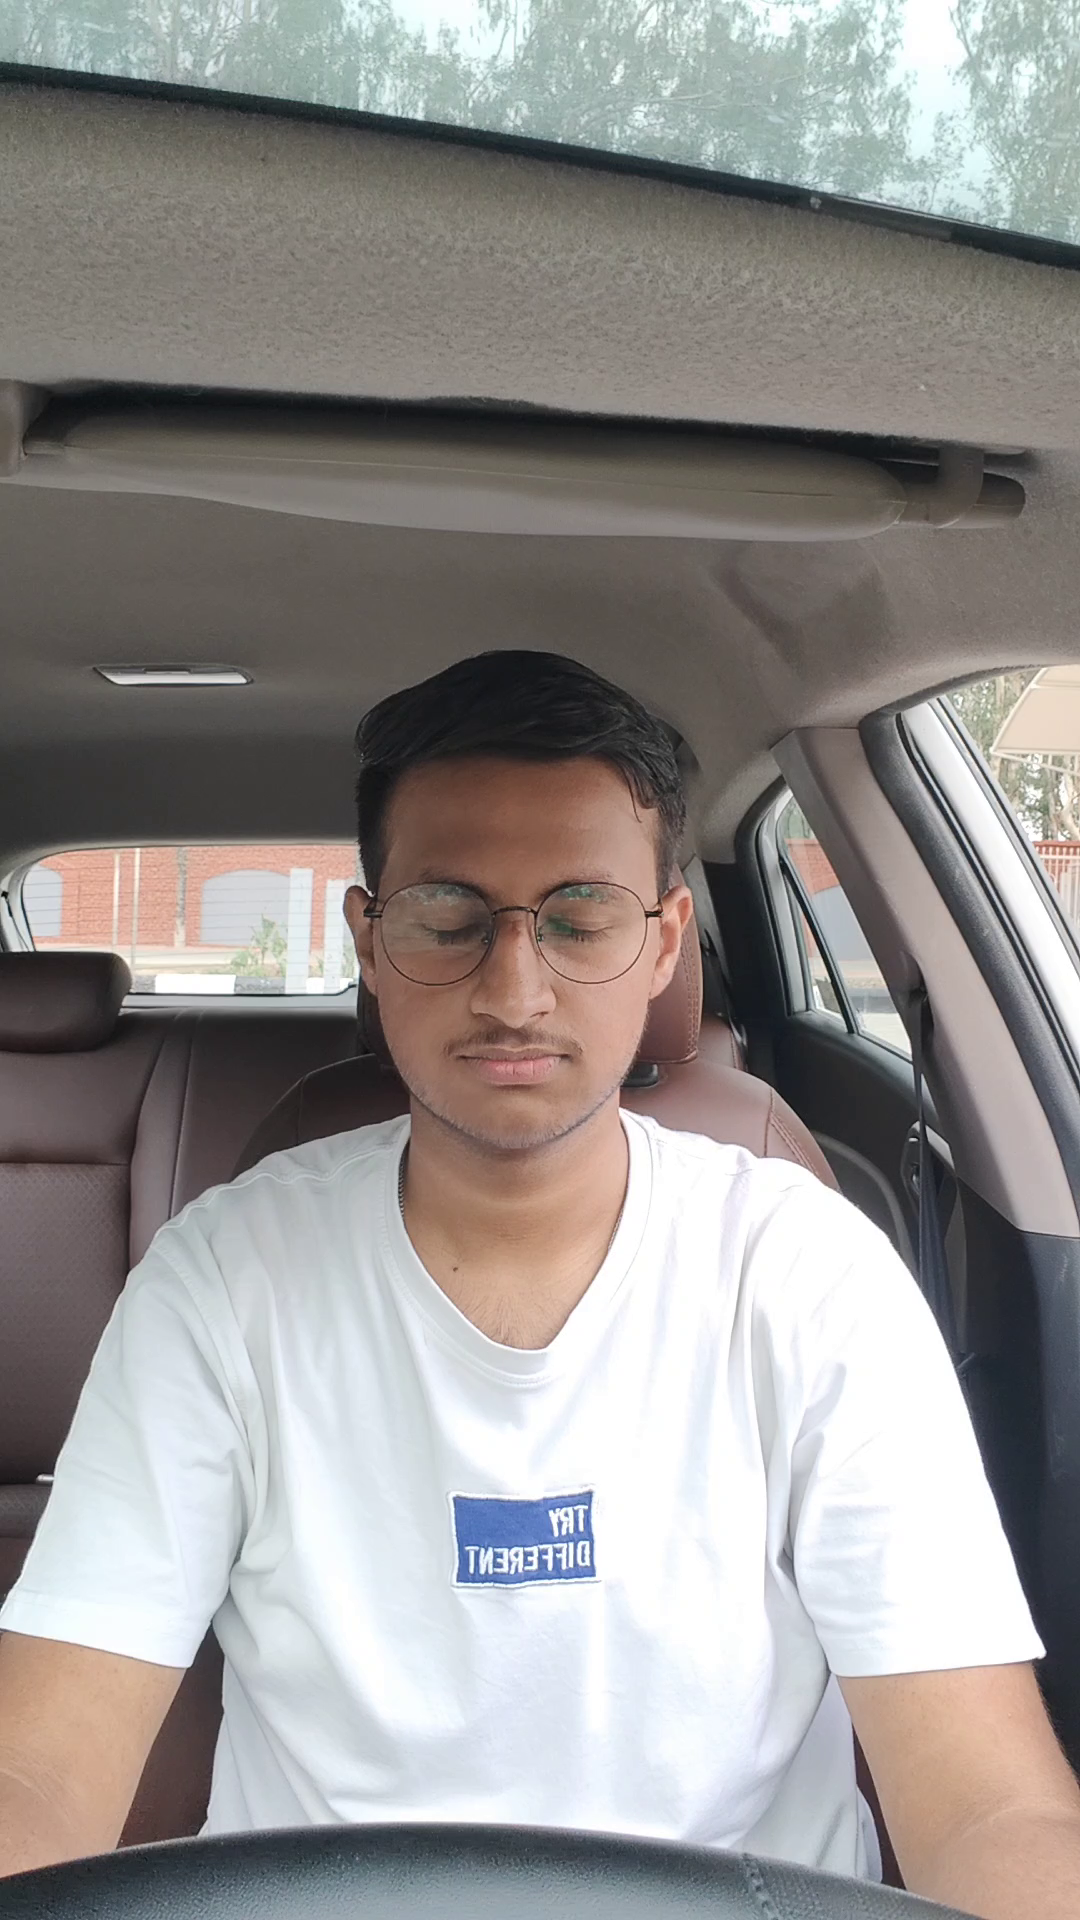
\includegraphics[draft=false, width=8cm,height=8cm]{drowsy.png}};

% Define explicit anchor for `input-east`
\coordinate (input-east) at ($(input.east) + (1,0,0)$);
\pic[shift={ (0,0,0) }] at (input-east) 
    {RightBandedBox={
        name=ccr_b1,
        caption= ,
        xlabel={{ 64, 64 }},
        zlabel=224,
        fill=\ConvColor,
        bandfill=\ConvReluColor,
        height=40,
        width={ 2.5 , 2.5 },
        depth=40
        }
    };

\pic[shift={ (0,0,0) }] at (ccr_b1-east) 
    {Box={
        name=pool_b1,
        caption= ,
        fill=\PoolColor,
        opacity=0.5,
        height=30,
        width=1,
        depth=30
        }
    };

\draw [connection]  (input-east)    -- node {\midarrow} (ccr_b1-west);

\pic[shift={ (1,0,0) }] at (pool_b1-east) 
    {RightBandedBox={
        name=ccr_b2,
        caption= ,
        xlabel={{ 128, 128 }},
        zlabel=112,
        fill=\ConvColor,
        bandfill=\ConvReluColor,
        height=32,
        width={ 3.5 , 3.5 },
        depth=32
        }
    };

\pic[shift={ (0,0,0) }] at (ccr_b2-east) 
    {Box={
        name=pool_b2,
        caption= ,
        fill=\PoolColor,
        opacity=0.5,
        height=24,
        width=1,
        depth=24
        }
    };

\draw [connection]  (pool_b1-east)    -- node {\midarrow} (ccr_b2-west);

\pic[shift={ (1,0,0) }] at (pool_b2-east) 
    {RightBandedBox={
        name=ccr_b31,
        caption= ,
        xlabel={{ 256, 256 }},
        zlabel=56,
        fill=\ConvColor,
        bandfill=\ConvReluColor,
        height=25,
        width={ 4.5 , 4.5 },
        depth=25
        }
    };

\pic[shift={ (0,0,0) }] at (ccr_b31-east) 
    {RightBandedBox={
        name=ccr_b32,
        caption= ,
        xlabel={{ 256, 256 }},
        zlabel=56,
        fill=\ConvColor,
        bandfill=\ConvReluColor,
        height=25,
        width={ 4.5 , 4.5 },
        depth=25
        }
    };

\pic[shift={ (0,0,0) }] at (ccr_b32-east) 
    {RightBandedBox={
        name=ccr_b33,
        caption= ,
        xlabel={{ 256, 256 }},
        zlabel=56,
        fill=\ConvColor,
        bandfill=\ConvReluColor,
        height=25,
        width={ 4.5 , 4.5 },
        depth=25
        }
    };

\pic[shift={ (0,0,0) }] at (ccr_b33-east) 
    {RightBandedBox={
        name=ccr_b34,
        caption= ,
        xlabel={{ 256, 256 }},
        zlabel=56,
        fill=\ConvColor,
        bandfill=\ConvReluColor,
        height=25,
        width={ 4.5 , 4.5 },
        depth=25
        }
    };

\pic[shift={ (0,0,0) }] at (ccr_b34-east) 
    {Box={
        name=pool_b3,
        caption= ,
        fill=\PoolColor,
        opacity=0.5,
        height=20.0,
        width=1,
        depth=20.0
        }
    };

\pic[shift={ (1,0,0) }] at (pool_b3-east) 
    {RightBandedBox={
        name=ccr_b41,
        caption= ,
        xlabel={{ 512, 512 }},
        zlabel=28,
        fill=\ConvColor,
        bandfill=\ConvReluColor,
        height=16,
        width={ 5.5 , 5.5 },
        depth=16
        }
    };

\pic[shift={ (0,0,0) }] at (ccr_b41-east) 
    {RightBandedBox={
        name=ccr_b42,
        caption= ,
        xlabel={{ 512, 512 }},
        zlabel=28,
        fill=\ConvColor,
        bandfill=\ConvReluColor,
        height=16,
        width={ 5.5 , 5.5 },
        depth=16
        }
    };

\pic[shift={ (0,0,0) }] at (ccr_b42-east) 
    {RightBandedBox={
        name=ccr_b43,
        caption= ,
        xlabel={{ 512, 512 }},
        zlabel=28,
        fill=\ConvColor,
        bandfill=\ConvReluColor,
        height=16,
        width={ 5.5 , 5.5 },
        depth=16
        }
    };

\pic[shift={ (0,0,0) }] at (ccr_b43-east) 
    {RightBandedBox={
        name=ccr_b44,
        caption= ,
        xlabel={{ 512, 512 }},
        zlabel=28,
        fill=\ConvColor,
        bandfill=\ConvReluColor,
        height=16,
        width={ 5.5 , 5.5 },
        depth=16
        }
    };

\pic[shift={ (0,0,0) }] at (ccr_b44-east) 
    {Box={
        name=pool_b4,
        caption= ,
        fill=\PoolColor,
        opacity=0.5,
        height=12.8,
        width=1,
        depth=12.8
        }
    };

\pic[shift={ (1,0,0) }] at (pool_b4-east) 
    {RightBandedBox={
        name=ccr_b51,
        caption= ,
        xlabel={{ 512, 512 }},
        zlabel=14,
        fill=\ConvColor,
        bandfill=\ConvReluColor,
        height=16,
        width={ 5.5 , 5.5 },
        depth=16
        }
    };

\pic[shift={ (0,0,0) }] at (ccr_b51-east) 
    {RightBandedBox={
        name=ccr_b52,
        caption= ,
        xlabel={{ 512, 512 }},
        zlabel=14,
        fill=\ConvColor,
        bandfill=\ConvReluColor,
        height=16,
        width={ 5.5 , 5.5 },
        depth=16
        }
    };

\pic[shift={ (0,0,0) }] at (ccr_b52-east) 
    {RightBandedBox={
        name=ccr_b53,
        caption= ,
        xlabel={{ 512, 512 }},
        zlabel=14,
        fill=\ConvColor,
        bandfill=\ConvReluColor,
        height=16,
        width={ 5.5 , 5.5 },
        depth=16
        }
    };

\pic[shift={ (0,0,0) }] at (ccr_b53-east) 
    {RightBandedBox={
        name=ccr_b54,
        caption= ,
        xlabel={{ 512, 512 }},
        zlabel=14,
        fill=\ConvColor,
        bandfill=\ConvReluColor,
        height=16,
        width={ 5.5 , 5.5 },
        depth=16
        }
    };

\pic[shift={ (0,0,0) }] at (ccr_b54-east) 
    {Box={
        name=pool_b5,
        caption= ,
        fill=\PoolColor,
        opacity=0.5,
        height=12.8,
        width=1,
        depth=12.8
        }
    };

\pic[shift={(2,0,0)}] at (pool_b5-east) 
    {Box={
        name=flatten,
        caption=Flatten,
        zlabel=7,
        fill=\SoftmaxColor,
        height=1,
        width=1,
        depth=40
        }
    };

\draw [connection]  (pool_b5-east)    -- node {\midarrow} (flatten-west);

\pic[shift={(1,0,0)}] at (flatten-east) 
    {Box={
        name=fc1,
        caption=Dense 512,
        zlabel=1,
        fill=\SoftmaxColor,
        height=1,
        width=1,
        depth=30
        }
    };

\draw [connection]  (flatten-east)    -- node {\midarrow} (fc1-west);

\pic[shift={(1,0,0)}] at (fc1-east) 
    {Box={
        name=fc2,
        caption=Dense Softmax,
        zlabel=1,
        fill=\SoftmaxColor,
        height=1,
        width=1,
        depth=20
        }
    };

\draw [connection]  (fc1-east)    -- node {\midarrow} (fc2-west);

\pic[shift={(1,0,0)}] at (fc2-east) 
    {Box={
        name=softmax,
        caption=Output,
        xlabel={{" ","dummy"}},
        zlabel=5,
        fill=\SoftmaxColor,
        opacity=0.8,
        height=3,
        width=1.5,
        depth=25
        }
    };

\draw [connection]  (fc2-east)    -- node {\midarrow} (softmax-west);

\end{tikzpicture}
\end{document}
